\chapter{Empurrando Juntos} \label{cap:empurrandojuntos}

O uso da tecnologia tem auxiliado no aumento da participação dos 
cidadãos no âmbito político e social de diversas maneiras. Discussões em sites, principalmente redes sociais, têm sido
destaques como uma forma recorrente desta participação \cite{marques2008participaccao}.
Contudo, considerando as características das plataformas utilizadas e a existência de grupos dominantes, interessados
na área passaram a observar um viés nas mensagens trocadas \cite{empurrandojuntos, marques2008participaccao}. 

O ``Empurrando Juntos'' surge nesse contexto, como uma plataforma capaz de contornar a situação de polarização nas discussões.
A ideia apresentada pelo Instituto Cidade Democrátiva tem como objetivo dar voz para a minoria e 
melhorar a efetividade dos debates e conversas de acordo com o seu propósito, possibilitando ao usuário
identificar grupos de opinião e tendências em uma conversa \cite{empurrandojuntos}. 

\begin{figure}[h!]
\centering
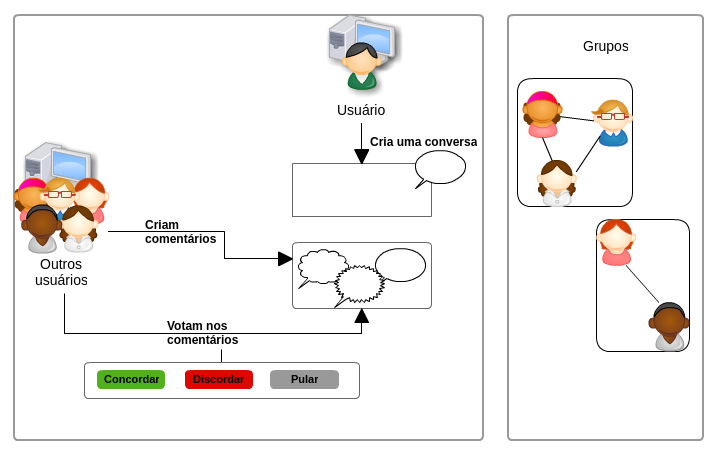
\includegraphics[scale=0.6]{figuras/resumo_ej.png}
\caption{Funcionamento do ``Empurrando Juntos''}
\label{fig:resumo_ej}
\end{figure}

A Figura \ref{fig:resumo_ej} ilustra o funcionamento completo do sistema. O usuário entra no sistema e pode criar conversas ou
comentar em conversas criadas por outros usuários. Para cada comentário realizado nessas conversas, é possível atribuir um 
``voto'' de concordância ou discordância do conteúdo exposto. Os votos são entendidos como a opinião dos usuários e são
utilizados para a formação dos grupos de opiniões. 

Em suma, o objetivo da plataforma é realizar o agrupamento de 
pessoas que responderam de maneira parecida, ou seja, concordaram e discordaram dos mesmos comentários.
Com os grupos formados, é possível ver a convergência e divergência de opiniões e assim
obter uma visualização mais efetiva da opinião das pessoas. 
